\section{函数解析的充要条件}

\subsection{柯西-黎曼方程}
\begin{frame}{可导函数的特点}
	\begin{itemize}
		\item 通过对一些简单函数的分析, 我们发现可导的函数往往可以直接表达为 $z$ 的函数的形式, 而不解析的往往包含 $x,y,\ov z$ 等内容.
		\item 这种现象并不是偶然的.
		\item 我们来研究二元实变量函数的可微性与复变函数可导的关系.
		\item 为了简便我们用 $u_x,u_y,v_x,v_y$ 等记号表示偏导数.
	\end{itemize}
\end{frame}


\begin{frame}{可导的等价刻画: 形式推导}
	\begin{itemize}
		\item 设 \alert{$f$ 在 $z$ 处可导}, $f'(z)=a+b\ii$,
		\item 则
		\[
			\Delta u+\ii\Delta v
			=\Delta f
			=(a+b\ii)(\Delta x+\ii\Delta y)+o(\Delta z).
		\]
		\item 展开可知
		\begin{align*}
			\Delta u&=a\Delta x-b\Delta y+o(\Delta z),\\
			\Delta v&=b\Delta x+a\Delta y+o(\Delta z).
		\end{align*}
		\item 由于 $o(\Delta z)=o(|\Delta z|)=o(\sqrt{x^2+y^2})$,
		\item 因此 \alert{$u,v$ 可微且 $u_x=v_y=a,v_x=-u_y=b$}.
	\end{itemize}
\end{frame}


\begin{frame}{可导的等价刻画: 形式推导}
	\begin{itemize}
		\item 反过来, 假设 \alert{$u,v$ 可微且 $u_x=v_y, v_x=-u_y$}.
		\item 由全微分公式
		\begin{align*}
			\Delta u&=u_x\Delta x+u_y\Delta y+o(\Delta z)
				=u_x\Delta x-v_x\Delta y+o(\Delta z),\\
				\visible<+->{\Delta v}&\visible<.->{=v_x\Delta x+v_y\Delta y+o(\Delta z)
				=v_x\Delta x+u_x\Delta y+o(\Delta z),}\\
			\visible<+->{\Delta f}&
			\visible<.->{=\Delta (u+\ii v)=(u_x+\ii v_x)\Delta x+(-v_x+\ii u_x)\Delta y}+o(\Delta z)\\
			&\visible<+->{=(u_x+\ii v_x)\Delta(x+\ii y)+o(\Delta z)}\\
			&\visible<+->{=(u_x+\ii v_x)\Delta z+o(\Delta z).}
		\end{align*}
		\item 故 \alert{$f(z)$ 在 $z$ 处可导, 且 $f'(z)=u_x+\ii v_x=v_y-\ii u_y$}.
	\end{itemize}
\end{frame}


\begin{frame}{可导的等价刻画: 柯西-黎曼方程}
	\begin{itemize}
		\item 由此得到
	\end{itemize}
	\onslide<+->
	\begin{theorem*}[][柯西-黎曼定理]
		$f(z)$ 在 $z$ 可导当且仅当\alert{在 $z$ 点 $u,v$ 可微}且满足\alert{柯西-黎曼方程} (简称为 C-R 方程):
		\[
			u_x=v_y,\quad v_x=-u_y.
		\]
		此时
		\[
			f'(z)=u_x+\ii v_x=v_y-\ii u_y.
		\]
	\end{theorem*}
	\onslide<+->
	\begin{center}
		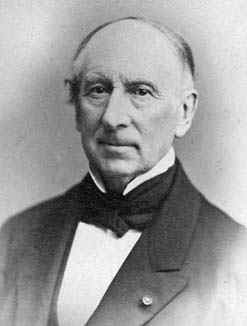
\includegraphics[height=25mm]{../image/Cauchy.jpeg}
		\hspace{2cm}
		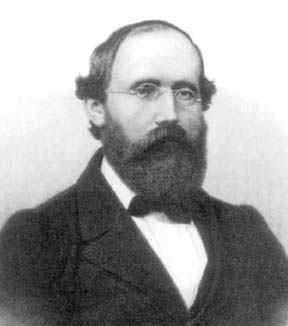
\includegraphics[height=25mm]{../image/Riemann.jpeg}
	\end{center}
\end{frame}


\begin{frame}{柯西-黎曼方程的等价形式\noexer}
	\begin{itemize}
		\item 注意到 $x=\dfrac12z+\dfrac12\ov z,y=-\dfrac \ii2z+\dfrac \ii2\ov z$.
		\item 仿照着二元实函数偏导数在变量替换下的变换规则, 定义 $f$ 对 $z$ 和 $\ov z$ 的偏导数为
		\[
			\laeq{\displaystyle
			\pp fz
			=\pp xz\pp fx+\pp yz\pp fy
			=\frac12\pp fx-\frac i2\pp fy,\\\displaystyle
			\pp f{\ov z}
			=\pp x{\ov z}\pp fx+\pp y{\ov z}\pp fy
			=\frac12\pp fx+\frac i2\pp fy.
			}.
		\]
		\item 若把 $z,\ov z$ 看成独立变量, 那么当 $f$ 在 $z$ 处可导时, $\diff f=f'\diff z$.
		\item 当 $f$ 关于 $z,\ov z$ 可微时(即 $u,v$ 可微), $\displaystyle\diff f=\pp fz\diff z+\pp f{\ov z}\diff\ov z$.
		\item 所以 \alert{$f$ 在 $z$ 处可导当且仅当 $u,v$ 可微且 $\dpp f{\ov z}=0$, 此时 $f'(z)=\dpp fz$.}
		\item 这也解释了为何含有 $x,y,\ov z$ 形式的函数往往不可导, 而可导的函数往往可以直接表达为 $z$ 的形式.
	\end{itemize}
\end{frame}


\begin{frame}{可导的充分性条件}
	\begin{itemize}
		\item 由于二元函数的偏导数均连续蕴含可微, 因此我们有:
	\end{itemize}
	\onslide<+->
	\begin{theorem}
		\begin{itemize}
			\item 若 $u_x,u_y,v_x,v_y$ 在 $z$ 处连续, 且满足C-R方程, 则 $f(z)$ 在 $z$ 可导.
			\item 若 $u_x,u_y,v_x,v_y$ 在区域 $D$ 上处处连续, 且满足C-R方程, 则 $f(z)$ 在 $D$ 上可导(从而解析).
		\end{itemize}
	\end{theorem}
	\begin{itemize}
		\item 这些连续性要求也可以换成 $\displaystyle \pdv fz$, $\displaystyle \pdv f{\ov z}$ 的连续性.
		\item 另外需要注意的是: \alert{柯西-黎曼定理中中的可微性和C-R方程缺一不可}.
	\end{itemize}
\end{frame}


\subsection{柯西-黎曼方程的应用}
\begin{frame}{典型例题: 利用C-R方程判断可导和解析}
	\onslide<+->
	\begin{example}[nearnext]
		函数 $f(z)=\ov z$ 在何处可导, 在何处解析?
	\end{example}
	\onslide<+->
	\begin{solution}[nearprev]
		\begin{itemize*}
			\item 由 $u=x,v=-y$ 可知
			\begin{align*}
				u_x&=1,&u_y&=0,\\
				v_x&=0,&v_y&=-1.
			\end{align*}
			\item 因为 $u_x=1\neq v_y=-1$, 所以该函数处处不可导, 处处不解析.
			\item 也可由 $\dpp f{\ov z}=1\neq0$ 看出.
		\end{itemize*}
	\end{solution}
\end{frame}


\begin{frame}{典型例题: 利用C-R方程判断可导和解析}
	\onslide<+->
	\begin{example}[near]
		函数 $f(z)=z\Re z$ 在何处可导, 在何处解析?
	\end{example}
	\onslide<+->
	\begin{solution}[near]
		\begin{itemize*}
			\item 由 $f(z)=x^2+\ii xy,u=x^2,v=xy$ 可知
			\item \begin{align*}
				u_x&=2x,&u_y&=0,\\
				v_x&=y, &v_y&=x.
			\end{align*}
			\item 由 $2x=x,0=-y$ 可知只有 $x=y=0,z=0$ 满足C-R方程.
			\item 因此该函数只在 $0$ 可导, 处处不解析且 $f'(0)=u_x(0)+\ii v_x(0)=0$.
			\item 也可由 $f=\dfrac12 z(z+\ov z), \dpp f{\ov z}=\dfrac12 z$ 看出, $f'(0)=\dpp fz\Big|_{z=0}=z|_{z=0}=0$.\smalldel
		\end{itemize*}
	\end{solution}
	\onslide<+->
\end{frame}


\begin{frame}{典型例题: 利用C-R方程判断可导和解析}
	\onslide<+->
	\begin{example}[near]
		函数 $f(z)=\ee^x(\cos y+\ii\sin y)$ 在何处可导, 在何处解析?
	\end{example}
	\onslide<+->
	\begin{solution}[near]
		\begin{itemize*}
			\item 由 $u=\ee^x\cos y,v=\ee^x\sin y$ 可知
			\item 
			\begin{align*}
				u_x&=\ee^x\cos y,&u_y&=-\ee^x\sin y,\\
				v_x&=\ee^x\sin y,&v_y&=\ee^x\cos y.
			\end{align*}
			\item 因此该函数处处可导, 处处解析, 且
			\[
				f'(z)=u_x+\ii v_x=\ee^x(\cos y+\ii\sin y)=f(z).
			\]
			\item 实际上, 这个函数就是复变量的指数函数 $\ee^z$.
			\meddel
		\end{itemize*}
	\end{solution}
\end{frame}


\begin{frame}{典型例题: 利用C-R方程判断可导和解析}
	\onslide<+->
	\begin{exercise}[nearnext]
		函数\fillbraceframe{A}在 $z=0$ 处不可导.
		\begin{exchoice}(2)
			() $2x+3yi$
			() $2x^2+3y^2\ii$
			() $\ee^x\cos y+\ii \ee^x\sin y$
			() $x^2-xyi$
		\end{exchoice}
	\end{exercise}
	\onslide<+->
	\begin{answer}[nearprev]
		\begin{itemize*}
			\item 根据C-R方程可知对于A, $u_x(0)=2\neq v_y(0)=3$.
			\item 对于BD, 各个偏导数在 $0$ 处取值都是 $0$.
			\item C则是处处都可导.
		\end{itemize*}
	\end{answer}
\end{frame}


\begin{frame}{例: 利用C-R方程判断可导和解析}
	\onslide<+->
	\begin{example}[nearnext]
		设函数 $f(z)=(x^2+axy+by^2)+\ii(cx^2+dxy+y^2)$ 在复平面内处处解析. 求实常数 $a,b,c,d$ 以及 $f'(z)$.
	\end{example}
	\onslide<+->
	\begin{solution}[nearprev]
		\begin{itemize*}
			\item 由于
			\bigdel
			\begin{align*}
				u_x&=2x+ay,&u_y=ax+2by,\\
				v_x&=2cx+dy,&v_y=dx+2y,
			\end{align*}
			\item 因此
			\[
				2x+ay=dx+2y,\quad ax+2by=-(2cx+dy),
			\]
			\item \centering $a=d=2,\quad b=c=-1$,
			\item \centering $f'(z)=u_x+\ii v_x=2x+2y+\ii(-2x+2y)=(2-2\ii)z$.
		\end{itemize*}
	\end{solution}
\end{frame}


\begin{frame}[<*>]{例: 利用C-R方程证明解析函数结论}
	\onslide<+->
	\begin{example}[nearnext]
		若 $f'(z)$ 在区域 $D$ 内处处为零, 则 $f(z)$ 在 $D$ 内是一常数.
	\end{example}
	\onslide<+->
	\begin{proof}[nearprev]
		\begin{itemize*}
			\item 由于 $f'(z)=u_x+\ii v_x=v_y-\ii u_y=0$,
			\item 因此 $u_x=v_x=u_y=v_y=0$, $u,v$ 均为常数,
			\item 从而 $f(z)=u+\ii v$ 是常数.\qedhere
		\end{itemize*}
	\end{proof}

	\onslide<+->
	类似地可以证明, 若 $f(z)$ 在 $D$ 内解析, 则下述条件均可推出 $f(z)$ 是常数:
	\onslide<+->
	\begin{figure}[hbpt]
		\begin{minipage}{0.48\textwidth}
			\begin{itemize}
				\item $\arg{f(z)}$ 是一常数,
				\item $\Re{f(z)}$ 是一常数,
				\item $v=u^2$.
			\end{itemize}
		\end{minipage}
		\begin{minipage}{0.48\textwidth}
			\begin{itemize}
				\item $|f(z)|$ 是一常数,
				\item $\Im{f(z)}$ 是一常数,
				\item $u=v^2$.
			\end{itemize}
		\end{minipage}
	\end{figure}
\end{frame}


\begin{frame}{例: 解析函数的保角性\noexer}
	\onslide<+->
	\begin{example}[near]
		若 $f(z)$ 解析且 $f'(z)$ 处处非零, 则曲线族 $u(x,y)=c_1$ 和曲线族 $v(x,y)=c_2$ 互相正交.
	\end{example}
	\onslide<+->
	\begin{proof}[near]
		\begin{itemize*}
			\item 由于 $f'(z)=u_x-\ii u_y$, 因此 $u_x,u_y$ 不全为零.
			\item 对 $u(x,y)=c_1$ 使用隐函数求导法则得 $u_x\diff x+u_y\diff y=0$,
			\item 从而 $(u_y,-u_x)$ 是该曲线在 $z$ 处的非零切向量.
		\end{itemize*}
		\begin{itemize*}
			\item 同理 $(v_y,-v_x)$ 是 $v(x,y)=c_2$ 在 $z$ 处的非零切向量.
			\item 由于
			\[
				u_yv_y+u_xv_x=u_yu_x-u_xu_y=0,
			\]
			\item 因此二者正交.\qedhere
			\meddel
		\end{itemize*}
	\end{proof}
\end{frame}


\begin{frame}{例: 解析函数的保角性\noexer}
	\begin{itemize}
		\item 当 $f'(z_0)\neq 0$ 时, 
		\item 经过 $z_0$ 的两条曲线 $C_1,C_2$ 的夹角和它们的像 $f(C_1),f(C_2)$ 在 $f(z_0)$ 处的夹角总是相同的.
		\item 这种性质被称为\emph{保角性}.
		\item 这是因为 $\diff f=f'(z_0)\diff z$.
		\item 局部来看 $f$ 把 $z_0$ 附近的点以 $z_0$ 为中心放缩 $f'(z_0)$ 倍并逆时针旋转 $\arg{f'(z_0)}$.
		\item 由 $w$ 复平面上曲线族 $u=c_1,v=c_2$ 正交可知上述例题成立.
	\end{itemize}
\end{frame}

